% homework/lab31/lab31.tex
% Year 7 - Science 3.1 Lab: Drop It!
%
% A FOUR-PAGE lab sheet (two A4 sheets, double-sided), one per student, used in
% class by groups of three. The teacher asked for it short: the first draft was
% 13 pages and was cut to this. Keep it at four. Results tables run sideways on
% purpose -- a vertical ten-drop table cost half a page.
%
% It lives in homework/ (like alg13) so the build script and the shelf work
% unchanged.
%
% THREE PARTS, ONE SPINE. Each part answers "how good is a stopwatch?" a little
% better, and together they answer the question 3.1 opened on, "do heavy things
% fall faster?":
%   Part 1  The ruler catch (3.1 slide 42, U03_lab slide 10). The ruler is the
%           accurate clock; the third student stopwatches the same fall and gets
%           numbers all over the place. Five catches each, a mean, a speed.
%   Part 2  Two objects, same size and shape, heavy and light, dropped from a
%           tape mark as high as the SHORTEST person can reach, so every Dropper
%           uses the same height. Two Timers, ten drops, jobs swapped.
%   Part 3  The same objects from the upstairs balcony. Height by long tape,
%           three readings. A one-second fall makes the 0.2 s reaction time
%           matter less (U03_lab slide 11, "Go higher").
%   Reflection: a letter to Aristotle (3.1 slide 6) written as claim, evidence,
%   reasoning.
%
% Nothing untaught: the mean is HW 9 / EX 9. Speed = distance / time is given in
% a remember box with Mr Bowen's example; calculators are allowed because
% dividing by a decimal is not Stage 7 arithmetic. 3.1 never says "air
% resistance" -- it says the air pushes up and slows it down. The ruler and
% fall-time tables are t = sqrt(2d / 10), the deck's own numbers.
%
% Build:  pwsh .claude/skills/new-homework/scripts/build-hw.ps1 lab31

\documentclass[12pt,a4paper]{article}

% -- Answer key switch -------------------------------------------------------
\newif\ifkey
\ifdefined\TEACHER\keytrue\else
  \keyfalse        % \keyfalse = student copy   |   \keytrue = teacher copy
\fi

% -- House style -------------------------------------------------------------
% homework/hw-style.tex
% Shared house style for every Year 7 homework packet. \input this from the
% packet file, right after \documentclass and the answer-key switch.
%
% Do not fork this file per packet. If a packet needs a different look, the
% question is whether every packet should have it.
%
% The choices here are deliberate and were arrived at by printing and looking:
%   * No solid dark banners. Every header is a light tint with a coloured spine
%     on the left, so colour reads clearly without flooding a school printer.
%   * No marks and no mark totals. These are practice, not exam papers.
%   * Lato at 12pt with open leading, plus mathastext so inline maths is Lato
%     too. Without mathastext every "-6 + 4" is Computer Modern serif and the
%     sheet looks half-typeset.
%   * Writing lines are spaced for Year 7 handwriting, not adult margin notes.
%   * Pages fill. \needspace is redefined below so a heading no longer drags
%     the page break up to itself, and every heading is glued to the box under
%     it. Packets built before 2026-09-30 were laid out under the old rules and
%     will reflow if rebuilt -- re-read every page if you rebuild one.
%
% Provides: \wlines \blank \tickbox \sep \qmk-free marks (none) \hwsection
% \qhead \expr, the workspace box, and the remember / wordhelp / activity /
% yourturn coloured boxes. Palette matches the lesson decks exactly.

% -- Packages ----------------------------------------------------------------
\usepackage[T1]{fontenc}
\usepackage[utf8]{inputenc}
\usepackage[default]{lato}
\usepackage[a4paper,top=1.7cm,bottom=1.7cm,left=2.0cm,right=2.0cm,headheight=15pt]{geometry}
\usepackage{amsmath,amssymb}
\usepackage{xcolor}
\usepackage[most]{tcolorbox}
\usepackage{enumitem}
\usepackage{tikz}
\usetikzlibrary{arrows.meta}
\usepackage{array}
\usepackage{tabularx}
\usepackage{fancyhdr}
\usepackage{multicol}
\usepackage{needspace}
\usepackage{graphicx}

% Make maths use Lato too. Without this, every "-6 + 4" on the page is set in
% Computer Modern serif and the sheet looks half-typeset. Must come last.
\usepackage[italic]{mathastext}

% -- \needspace, without the hole it used to leave ----------------------------
% needspace.sty writes "\vskip 0pt plus X \penalty-100" in front of every
% heading. A page that ends anywhere else is underfull with no stretch, so TeX
% scores it b=10000; a page that ends AT a heading gets that X of stretch and a
% finite badness, and wins. So any heading in roughly the bottom half of a page
% claimed the break, and the question under it moved over whole, leaving a hole
% the size of the question. \tracingpages showed it exactly (b=4531 at the
% heading, b=10000 at every later break) while building homework/q1rev, and it
% is where the half-empty pages in HW 1-8 came from.
% This keeps only the \penalty9999, which still refuses to put a heading in the
% last X of a page. Keeping a heading WITH the box under it is \nobreak's job
% now -- see \hwsection and \qhead below.
\makeatletter
\renewcommand{\needspace}[1]{\begingroup\setlength{\dimen@}{#1}%
  \vskip\dimen@\penalty9999\vskip-\dimen@\endgroup}
\makeatother

\linespread{1.06}\selectfont

% -- The Learner's Book palette (same hex values as the lesson decks) ---------
\definecolor{cbteal}{HTML}{0087A8}
\definecolor{cbpurple}{HTML}{5C2483}
\definecolor{cborange}{HTML}{C25E12}
\definecolor{cbgreen}{HTML}{4A8B23}
\definecolor{cbred}{HTML}{C8102E}
\definecolor{cbblue}{HTML}{1A5FA8}
\definecolor{rulegray}{HTML}{9AA5AD}

% -- Answer lines and blanks -------------------------------------------------
% \wlines{n} draws n ruled writing lines, spaced wide enough for Year 7
% handwriting rather than for an adult with a fine pen.
\makeatletter
\newcommand{\wlines}[1]{%
  \par\vspace{0.75em}%
  \@tempcnta=0\relax
  \@whilenum\@tempcnta<#1\do{%
    \hbox to \linewidth{\color{rulegray}\leaders\hrule height 0.5pt\hfill}%
    \vspace{1.5em}%
    \advance\@tempcnta by 1\relax}%
  \par\vspace{-0.8em}%
}
\makeatother

% \blank[width] is an inline gap to write a short answer in.
\newcommand{\blank}[1][2.6cm]{\underline{\hspace{#1}}}

% A boxed space for showing working.
\newtcolorbox{workspace}[1][3.4cm]{%
  colback=white, colframe=rulegray, boxrule=0.5pt, arc=5pt,
  height=#1, left=6pt, right=6pt, top=4pt, bottom=4pt,
  before skip=9pt, after skip=11pt}

% An empty tick box.
\newcommand{\tickbox}{\fbox{\rule{0pt}{1.15em}\rule{1.15em}{0pt}}}

% A middot separator.
\newcommand{\sep}{\,\textperiodcentered\,}

% -- Section and question headings -------------------------------------------
% Light tint plus a fat coloured spine on the left. No solid dark banner: the
% colour reads clearly but barely costs the printer anything.
% needspace keeps a heading out of the last few lines of a page. The \nobreak
% after it keeps it with whatever comes next: a remember or word-help box that
% does not fit takes its heading over with it, instead of leaving the heading
% alone at the foot of the page. (The old needspace did that by accident, and
% left a hole every time; see above.)
\newcommand{\hwsection}[2][cbteal]{%
  \needspace{8\baselineskip}%
  \par\vspace{13pt}%
  \noindent
  \begin{tcolorbox}[enhanced, nobeforeafter, width=\textwidth,
      colback=#1!7, colframe=#1!7, arc=5pt,
      borderline west={5pt}{0pt}{#1},
      left=14pt, right=10pt, top=7pt, bottom=7pt]
    {\large\bfseries\color{#1}#2}
  \end{tcolorbox}%
  \par\nobreak\vspace{9pt}}

% \qhead[colour]{A2}{Moving along the line} -- a question heading.
\newcommand{\qhead}[3][cbteal]{%
  \needspace{6\baselineskip}%
  \par\vspace{11pt}%
  \noindent{\large\bfseries\color{#1}#2}\quad{\large\bfseries #3}\par\nobreak\vspace{4pt}}

% -- Coloured boxes ----------------------------------------------------------
% Shared look: rounded, light fill, coloured rule, coloured title text on a
% pale title strip rather than a dark one.
% NOT breakable. A breakable box that cannot fit its first lines forces its own
% page break, and \nobreak cannot stop a forced break -- so the heading above
% it was left alone at the foot of the page (tested: it happens with \nobreak
% in place). Unbreakable, the page builder moves heading and box together.
% These boxes are a few lines each; none needs to split.
\tcbset{hwbox/.style={
  enhanced, arc=6pt, boxrule=1pt,
  left=11pt, right=11pt, top=8pt, bottom=8pt,
  fonttitle=\bfseries, attach boxed title to top left={xshift=12pt, yshift=-8pt},
  boxed title style={arc=4pt, boxrule=1pt, left=7pt, right=7pt, top=2pt, bottom=2pt},
  top=13pt}}

% Orange: things to remember. Matches the deck's "Write This Down".
\newtcolorbox{remember}[1][Remember from the lesson]{hwbox,
  colback=cborange!6, colframe=cborange, coltitle=cborange,
  colbacktitle=white, title={#1}}

% Blue: English help. The barrier in this class is the wording, not the maths.
\newtcolorbox{wordhelp}[1][Word help]{hwbox,
  colback=cbblue!6, colframe=cbblue, coltitle=cbblue,
  colbacktitle=white, title={#1}}

% Purple: an activity or instruction.
\newtcolorbox{activity}[1][How to do this homework]{hwbox,
  colback=cbpurple!6, colframe=cbpurple, coltitle=cbpurple,
  colbacktitle=white, title={#1}}

% Green: your turn / a friendly nudge.
\newtcolorbox{yourturn}[1][Your turn]{hwbox,
  colback=cbgreen!7, colframe=cbgreen, coltitle=cbgreen!75!black,
  colbacktitle=white, title={#1}}

% -- Shorthands --------------------------------------------------------------
\newcommand{\dC}{\,^{\circ}\mathrm{C}}          % use inside maths: $-8\dC$
\newcommand{\key}[1]{{\color{cborange}\textbf{#1}}}
\newcommand{\eng}[1]{{\color{cbblue}\textbf{#1}}}

\setlist[enumerate]{itemsep=8pt, topsep=5pt, leftmargin=*}
\setlist[itemize]{itemsep=4pt, topsep=4pt, leftmargin=*}
\renewcommand{\arraystretch}{1.45}

% -- An expression the student is asked to work from -------------------------
\newcommand{\expr}[1]{%
  \tcbox[on line, colback=cbgreen!10, colframe=cbgreen!55, boxrule=1pt, arc=4pt,
         left=9pt, right=9pt, top=4pt, bottom=4pt]{\large\bfseries $#1$}}

% -- Running head and foot ---------------------------------------------------
% The packet overrides \fancyhead[L] with its own title.
\pagestyle{fancy}
\fancyhf{}
\fancyhead[L]{\small\color{black!55}Year 7\sep Homework}
\fancyhead[R]{\small\color{black!55}Name: \blank[3.4cm]}
\fancyfoot[C]{\small\color{black!55}Page \thepage}
\renewcommand{\headrulewidth}{0pt}
\renewcommand{\headrule}{\vspace{2pt}\hbox to\headwidth{\color{cbteal!45}\leaders\hrule height 1.2pt\hfill}}


\usepackage{colortbl}   % \rowcolor for the table headers, \cellcolor for blanks

% A list straight after a heading must not be the place the page breaks: the
% default -51 before every list stranded a heading at the foot of a page.
\makeatletter\@beginparpenalty=\@M\makeatother

% -- Per-packet running head -------------------------------------------------
\fancyhead[L]{\small\color{black!55}Year 7\sep Science 3.1\sep Lab: Drop It!}

% -- Writing lines that will not be split ------------------------------------
\newcommand{\qlines}[1]{\par\needspace{\numexpr#1+1\relax\baselineskip}\wlines{#1}}

% -- Columns, rows and cells -------------------------------------------------
\newcolumntype{L}{>{\raggedright\arraybackslash}X}
\newcolumntype{Y}{>{\centering\arraybackslash}X}
\newcolumntype{C}[1]{>{\centering\arraybackslash}p{#1}}
\newcommand{\tall}{\rule[-0.55em]{0pt}{1.8em}}
\newcommand{\hrow}{\rowcolor{cbteal!10}}
\newcommand{\nocell}{\cellcolor{black!7}}

% -- A sentence starter: grey, so it reads as given, not as the answer --------
\newcommand{\starter}[1]{{\color{black!60}#1}}

% -- A job name, as a small teal tag ------------------------------------------
\newcommand{\job}[1]{\tcbox[on line, colback=cbteal!10, colframe=cbteal!70,
  boxrule=0.8pt, arc=3pt, left=3pt, right=3pt, top=0pt, bottom=0pt,
  boxsep=1pt]{\small\bfseries\color{cbteal!70!black}#1}}

% -- "Think", as a small purple tag: the one question at the end of each part --
\newcommand{\think}{\tcbox[on line, colback=cbpurple!10, colframe=cbpurple!70,
  boxrule=0.8pt, arc=3pt, left=3pt, right=3pt, top=0pt, bottom=0pt,
  boxsep=1pt]{\small\bfseries\color{cbpurple}Think}\ }

% -- The speed calculation, worded the same way in all three parts ------------
% #1 = what is moving, #2 = the distance in words.
\newcommand{\speedline}[2]{\par\noindent\textbf{Speed of #1} $=$ #2 $\div$ mean
  time $=$ \blank[1.5cm] $\div$ \blank[1.5cm] $=$ \blank[1.7cm] \textbf{m/s}\par}

% -- Red: safety. Same shape as the other house boxes. ------------------------
\newtcolorbox{safety}[1][Stay safe]{hwbox,
  colback=cbred!5, colframe=cbred, coltitle=cbred,
  colbacktitle=white, title={#1}}

% -- Tighter lists for the method steps ----------------------------------------
\newlist{steps}{enumerate}{1}
\setlist[steps]{label=\textbf{\arabic*.}, itemsep=1pt, topsep=2pt, leftmargin=*}

% -- Colours for the drawings -------------------------------------------------
\definecolor{skin}{HTML}{F1C9A5}
\definecolor{rulerfill}{HTML}{FFF3C4}
\definecolor{ink}{HTML}{2B2B2B}

% -- A 30 cm ruler, 0 at the bottom, 0.09 cm of page per cm of ruler ----------
\tikzset{
  rulerpic/.pic={
    \draw[fill=rulerfill, line width=0.8pt, draw=ink] (0,-0.1) rectangle (0.7,2.8);
    \foreach \c in {0,...,30} {\draw[line width=0.3pt, ink] (0,\c*0.09) -- (0.14,\c*0.09);}
    \foreach \c in {0,10,20,30} {\draw[line width=0.7pt, ink] (0,\c*0.09) -- (0.28,\c*0.09);
      \node[font=\tiny\bfseries, anchor=east, inner sep=1pt, text=ink] at (0.68,\c*0.09) {\c};}
  }}

% -- A stick figure with its feet at (#1,#2); arms are drawn separately -------
\newcommand{\stick}[2]{%
  \begin{scope}[shift={(#1,#2)}, line width=1.2pt, line cap=round, line join=round, draw=ink]
    \draw (-0.18,0) -- (0,0.55) -- (0.18,0);
    \draw (0,0.55) -- (0,1.08);
    \draw[fill=white] (0,1.26) circle (0.18);
  \end{scope}}

% -- A traffic cone with its base centred at (#1,#2) --------------------------
\newcommand{\cone}[2]{%
  \fill[cborange, draw=ink, line width=0.6pt] (#1-0.15,#2) -- (#1,#2+0.42) -- (#1+0.15,#2) -- cycle;}

\begin{document}

% ===========================================================================
% PAGE 1 -- COVER, SAFETY, PART 1 METHOD
% ===========================================================================
\thispagestyle{fancy}

\begin{tcolorbox}[enhanced, colback=cbpurple!7, colframe=cbpurple!7, arc=7pt,
                  borderline west={6pt}{0pt}{cbpurple},
                  left=16pt, right=12pt, top=7pt, bottom=7pt]
  \begin{minipage}[c]{0.78\linewidth}
    {\color{cbpurple}\bfseries YEAR 7\sep SCIENCE 3.1\sep LAB}\\[3pt]
    {\color{cbpurple}\Huge\bfseries Drop It!}\\[4pt]
    {\color{black!70}How fast are you? Do heavy things fall faster?}
  \end{minipage}\hfill
  % Two balls falling side by side, one dot every 0.1 s: the gaps grow because
  % they accelerate (the multi-flash photo from 3.1).
  \begin{minipage}[c]{0.18\linewidth}\centering
    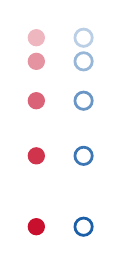
\begin{tikzpicture}[x=1cm, y=1cm]
      \foreach \t/\op in {1/0.3, 2/0.45, 3/0.65, 4/0.85, 5/1} {
        \fill[cbred, opacity=\op] (0, {0.1-0.1*\t*\t}) circle (0.11);
        \draw[cbblue, line width=1pt, fill=white, opacity=\op] (0.6, {0.1-0.1*\t*\t}) circle (0.11);
      }
    \end{tikzpicture}
  \end{minipage}
\end{tcolorbox}

\vspace{6pt}
\noindent\textbf{Name:} \blank[5.0cm] \hfill \textbf{Class:} \blank[2.6cm]
\hfill \textbf{Date:} \blank[3.4cm]

\vspace{8pt}
\noindent\textbf{My group:} \quad 1.\,\blank[3.9cm] \quad 2.\,\blank[3.9cm]
\quad 3.\,\blank[3.9cm]

\begin{yourturn}[Predict first --- on your own]
  Mr Bowen drops a heavy ball and a light ball, the same size, at the same time.
  Which lands first? \quad \tickbox\,\,heavy \quad\; \tickbox\,\,light
  \quad\; \tickbox\,\,same time

  \vspace{4pt}
  \noindent\starter{I think \ldots\ because \ldots}
  \wlines{1}
\end{yourturn}

\begin{safety}[Stay safe]
  \small
  \begin{multicols}{2}
  \begin{itemize}[itemsep=1pt, topsep=0pt]
    \item Only drop objects \textbf{Mr Bowen has checked}.
    \item \textbf{Let go. Never throw. Never catch.}
    \item Part 2: feet on the floor. No chairs or desks.
    \columnbreak
    \item Part 3: stay \textbf{behind the railing}. Never lean.
    \item Part 3: drop only after the Ground person shouts \textbf{``Clear!''}
  \end{itemize}
  \end{multicols}
\end{safety}

\begin{remember}[Two tools: you can use a calculator]
  \key{Mean} $=$ add up all the values, then divide by how many there are.

  \vspace{3pt}
  \key{Speed $=$ distance $\div$ time}, in \key{m/s} (\eng{metres per second}).
  \quad \key{cm to m:} $\div\ 100$

  \vspace{3pt}
  Mr Bowen: 20 cm $=$ 0.20 m, in 0.20 s, so speed $= 0.20 \div 0.20 =
  \mathbf{1.0}$ \textbf{m/s}.
\end{remember}

% ===========================================================================
% PART 1 -- THE RULER CATCH
% ===========================================================================
\hwsection{Part 1 \textperiodcentered\ The Ruler Catch --- How Fast Are You?}

\noindent
\begin{minipage}[c]{0.66\textwidth}
  \textbf{Jobs:} \job{Catcher} \job{Dropper} \job{Timer}
  \begin{steps}
    \item \textbf{Catcher:} rest your arm on the desk. Thumb and finger open, at
          the \textbf{0}.
    \item \textbf{Dropper:} hold the top. Let go with \key{\mbox{no countdown}}!
    \item \textbf{Catcher:} catch it. Read the cm at the \textbf{top of your
          thumb}.
    \item \textbf{Timer:} try to time the fall with a stopwatch.
    \item \textbf{5 catches each.} Then change jobs.
  \end{steps}
\end{minipage}\hfill
\begin{minipage}[c]{0.31\textwidth}\centering
  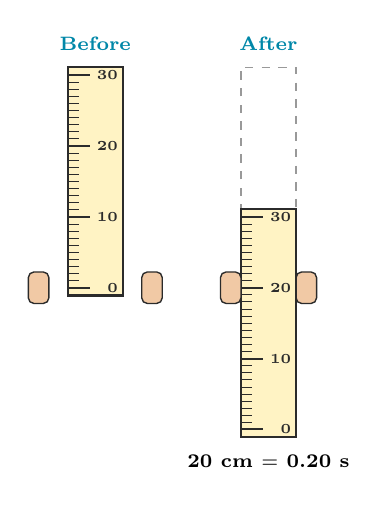
\begin{tikzpicture}[x=1cm, y=1cm, font=\scriptsize]
    % BEFORE: fingers open at 0
    \node[font=\scriptsize\bfseries, text=cbteal] at (0.35,3.1) {Before};
    \pic at (0,0) {rulerpic};
    \fill[skin, draw=ink, line width=0.5pt, rounded corners=2pt] (-0.5,-0.2) rectangle (-0.24,0.2);
    \fill[skin, draw=ink, line width=0.5pt, rounded corners=2pt] (0.94,-0.2) rectangle (1.2,0.2);
    % AFTER: caught at 20 cm
    \begin{scope}[xshift=2.2cm]
      \node[font=\scriptsize\bfseries, text=cbteal] at (0.35,3.1) {After};
      \draw[black!40, dashed, line width=0.5pt] (0,-0.1) rectangle (0.7,2.8);
      \pic at (0,-1.8) {rulerpic};
      \fill[skin, draw=ink, line width=0.5pt, rounded corners=2pt] (-0.26,-0.2) rectangle (0,0.2);
      \fill[skin, draw=ink, line width=0.5pt, rounded corners=2pt] (0.7,-0.2) rectangle (0.96,0.2);
      \node[anchor=north, font=\scriptsize\bfseries, align=center] at (0.35,-2.0) {20 cm $=$ 0.20 s};
    \end{scope}
  \end{tikzpicture}
\end{minipage}

% -- 1A ---------------------------------------------------------------------
% The deck's table (3.1 slide 42) in 1-cm steps: t = sqrt(2d/10), d in metres.
\qhead{1A}{The ruler table: where you caught it $\rightarrow$ your reaction time}

\noindent\begin{minipage}{\textwidth}
\centering\small
\setlength{\tabcolsep}{3pt}%
\renewcommand{\arraystretch}{1.2}%
\begin{tabular}{|l|*{10}{C{1.02cm}|}}
  \hline
  \hrow \textbf{Caught at (cm)} & 1 & 2 & 3 & 4 & 5 & 6 & 7 & 8 & 9 & 10 \\ \hline
  \textbf{Time (s)} & 0.04 & 0.06 & 0.08 & 0.09 & 0.10 & 0.11 & 0.12 & 0.13 & 0.13 & 0.14 \\ \hline
  \hrow \textbf{Caught at (cm)} & 11 & 12 & 13 & 14 & 15 & 16 & 17 & 18 & 19 & 20 \\ \hline
  \textbf{Time (s)} & 0.15 & 0.15 & 0.16 & 0.17 & 0.17 & 0.18 & 0.18 & 0.19 & 0.19 & 0.20 \\ \hline
  \hrow \textbf{Caught at (cm)} & 21 & 22 & 23 & 24 & 25 & 26 & 27 & 28 & 29 & 30 \\ \hline
  \textbf{Time (s)} & 0.20 & 0.21 & 0.21 & 0.22 & 0.22 & 0.23 & 0.23 & 0.24 & 0.24 & 0.24 \\ \hline
\end{tabular}
\end{minipage}

% -- 1B ---------------------------------------------------------------------
\qhead{1B}{My five catches}

\noindent\begin{minipage}{\textwidth}
\small
\setlength{\tabcolsep}{4pt}%
\begin{tabularx}{\textwidth}{|C{3.5cm}|Y|Y|Y|Y|Y|C{1.6cm}|C{1.9cm}|}
  \hline
  \hrow \textbf{Catch} & \textbf{1} & \textbf{2} & \textbf{3} & \textbf{4} &
  \textbf{5} & \textbf{Total} & \textbf{Mean} ($\div\,5$) \\ \hline
  \textbf{Caught at (cm)} \tall & & & & & & & \\ \hline
  \textbf{Ruler time (s)} \tall & & & & & & & \\ \hline
  \textbf{Stopwatch time (s)} \tall & & & & & & & \\ \hline
\end{tabularx}
\end{minipage}

\vspace{10pt}
\speedline{the ruler}{mean catch (m)}

\vspace{8pt}
\noindent\think Your ruler times and stopwatch times are different. Why is a
stopwatch no good for timing the ruler? Use \eng{reaction time}. \\
\starter{The fall only takes about \ldots\ The Timer \ldots}
\qlines{2}

% ===========================================================================
% PART 2 -- TWO OBJECTS IN THE LAB
% ===========================================================================
\hwsection{Part 2 \textperiodcentered\ Two Objects in the Lab --- Do Heavy Things
Fall Faster?}

\noindent\textbf{Our objects}, the \key{same size and shape}: \quad
\textbf{A} (heavy) \blank[2.9cm] \quad \textbf{B} (light) \blank[2.9cm]

\vspace{6pt}
\noindent\textbf{Jobs:} \job{Dropper} \job{Timer A} \job{Timer B} \hfill
{\small\color{black!70}Checked by Mr Bowen}\; \tickbox
\begin{steps}
  \item Put tape on the wall, as high as the \textbf{shortest} person can reach.
        Drop from this mark \key{every time}.
  \item Dropper: hold A and B at the tape. Say \textbf{``3, 2, 1, drop!''} and let
        go of both together.
  \item Timer A times A. Timer B times B. Everyone listens: \textbf{one bang or
        two?}
  \item Do \textbf{10 drops}. Change jobs after drop 3 and drop 6.
\end{steps}

\vspace{6pt}
\noindent\textbf{Height of the tape:} \blank[2.0cm] cm $=$ \blank[2.0cm] m

% -- 2A ---------------------------------------------------------------------
\qhead{2A}{Ten drops}

\noindent\begin{minipage}{\textwidth}
{\small Write each time like this: 0.63. Last row: who landed first? \textbf{A},
\textbf{B} or \textbf{S} (same time).}

\vspace{4pt}
\small
\setlength{\tabcolsep}{2pt}%
\begin{tabularx}{\textwidth}{|C{2.5cm}|*{10}{Y|}C{1.25cm}|C{1.35cm}|}
  \hline
  \hrow \textbf{Drop} & 1 & 2 & 3 & 4 & 5 & 6 & 7 & 8 & 9 & 10 & \textbf{Total} &
  \textbf{Mean} \\ \hline
  \textbf{A, heavy (s)} \tall & & & & & & & & & & & & \\ \hline
  \textbf{B, light (s)} \tall & & & & & & & & & & & & \\ \hline
  \textbf{First? A, B, S} \tall & & & & & & & & & & & \nocell & \nocell \\ \hline
\end{tabularx}
\end{minipage}

\vspace{10pt}
\speedline{A}{height (m)}

\vspace{8pt}
\noindent\think Why did we \textbf{change} Timers? Why must A and B be the same
size and shape? \\
\starter{So that a slow Timer \ldots\ If one is bigger or flatter, the air \ldots}
\qlines{2}

% ===========================================================================
% PART 3 -- THE BALCONY
% ===========================================================================
\hwsection{Part 3 \textperiodcentered\ From the Balcony --- How Fast Does It Go?}

\noindent
\begin{minipage}[c]{0.55\textwidth}
  \textbf{Upstairs:} \job{Dropper} \job{Timer A} \\[2pt]
  \textbf{Downstairs:} \job{Ground person}, who also times B
  \begin{steps}
    \item \textbf{Height:} the Ground person holds the \textbf{0} of the long tape
          on the ground. Upstairs, read it at the \textbf{top of the railing}.
          Three readings.
    \item The Ground person stands well back and shouts \textbf{``Clear!''}
    \item The Dropper holds A and B out over the railing, level with the top:
          \textbf{``3, 2, 1, drop!''}
    \item Timer A times A. The Ground person times B, then
          \textbf{walks} them back up.
    \item Change jobs after \key{every} drop. Do \textbf{6 drops}.
  \end{steps}
\end{minipage}\hfill
% Side view. 1 unit = about 1 m. Railing top at 4.2, the drop height.
\begin{minipage}[c]{0.42\textwidth}\centering
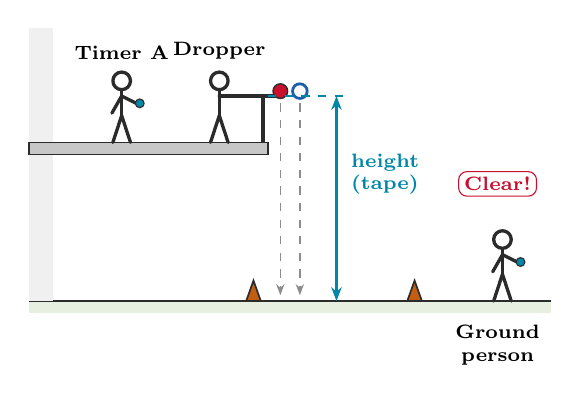
\begin{tikzpicture}[x=0.62cm, y=0.62cm, font=\scriptsize]
  \fill[cbgreen!14] (-0.3,-0.25) rectangle (10.4,0);
  \draw[ink, line width=0.9pt] (-0.3,0) -- (10.4,0);
  \fill[black!6] (-0.3,0) rectangle (0.2,5.6);
  \fill[black!22, draw=ink, line width=0.5pt] (-0.3,3.0) rectangle (4.6,3.25);
  \draw[ink, line width=1.4pt] (4.5,3.25) -- (4.5,4.2);
  \draw[ink, line width=1.4pt] (4.3,4.2) -- (4.6,4.2);
  % Timer A and the Dropper upstairs
  \stick{1.6}{3.25}
  \draw[ink, line width=1.2pt, line cap=round] (1.4,3.85) -- (1.6,4.2) -- (1.9,4.05);
  \fill[cbteal, draw=ink, line width=0.4pt] (1.97,4.05) circle (0.09);
  \stick{3.6}{3.25}
  \draw[ink, line width=1.2pt, line cap=round] (3.6,4.2) -- (4.75,4.2);
  \node[anchor=south, font=\scriptsize\bfseries] at (1.6,4.75) {Timer A};
  \node[anchor=south, font=\scriptsize\bfseries] at (3.6,4.75) {Dropper};
  % the objects and their fall
  \fill[cbred, draw=ink, line width=0.5pt] (4.85,4.3) circle (0.15);
  \draw[cbblue, line width=1pt, fill=white] (5.25,4.3) circle (0.15);
  \draw[black!45, dashed, line width=0.6pt, -{Stealth[length=4pt]}] (4.85,4.05) -- (4.85,0.12);
  \draw[black!45, dashed, line width=0.6pt, -{Stealth[length=4pt]}] (5.25,4.05) -- (5.25,0.12);
  % the height, from the top of the railing to the ground
  \draw[{Stealth[length=5pt]}-{Stealth[length=5pt]}, line width=1pt, cbteal] (6.0,0) -- (6.0,4.2);
  \draw[cbteal, dashed, line width=0.5pt] (4.6,4.2) -- (6.2,4.2);
  \node[anchor=west, text=cbteal, font=\scriptsize\bfseries, align=left] at (6.1,2.6) {height\\(tape)};
  % landing zone and the Ground person
  \cone{4.3}{0}
  \cone{7.6}{0}
  \stick{9.4}{0}
  \draw[ink, line width=1.2pt, line cap=round] (9.2,0.6) -- (9.4,0.95) -- (9.7,0.8);
  \fill[cbteal, draw=ink, line width=0.4pt] (9.77,0.8) circle (0.09);
  \node[draw=cbred, fill=white, rounded corners=3pt, text=cbred, font=\scriptsize\bfseries,
        inner sep=2pt] at (9.3,2.4) {Clear!};
  \node[anchor=north, font=\scriptsize\bfseries, align=center] at (9.3,-0.3) {Ground\\person};
\end{tikzpicture}
\end{minipage}

% -- 3A ---------------------------------------------------------------------
% Fall times with no air, g = 10: the deck's slide 43 numbers. Two ranges, so
% the one table serves Part 2 (a tape mark near 2 m) and Part 3 (one storey).
\qhead{3A}{Height and prediction}

\noindent\begin{minipage}{\textwidth}
\small
\setlength{\tabcolsep}{4pt}%
\begin{tabularx}{\textwidth}{|C{3.5cm}|Y|Y|Y|C{2.6cm}|}
  \hline
  \hrow & \textbf{Reading 1} & \textbf{Reading 2} & \textbf{Reading 3} &
  \textbf{Mean} ($\div\,3$) \\ \hline
  \textbf{Height (m)} \tall & & & & \\ \hline
\end{tabularx}

\vspace{8pt}
\noindent How long a fall takes with \textbf{no air}:

\vspace{3pt}
\centering
\setlength{\tabcolsep}{3pt}%
\renewcommand{\arraystretch}{1.2}%
\begin{tabular}{|l|*{11}{C{0.92cm}|}}
  \hline
  \hrow \textbf{Height (m)} & 1.8 & 2.0 & 2.2 & 3.0 & 3.5 & 4.0 & 4.5 & 5.0 & 5.5 & 6.0 & 7.0 \\ \hline
  \textbf{Time (s)} & 0.60 & 0.63 & 0.66 & 0.77 & 0.84 & 0.89 & 0.95 & 1.00 & 1.05 & 1.10 & 1.18 \\ \hline
\end{tabular}
\end{minipage}

\vspace{8pt}
\noindent\textbf{Predict.} From our height, the fall takes about \blank[1.8cm] s.

\vspace{6pt}
\noindent Which lands first from up here? \quad \tickbox\,\,A
\quad\; \tickbox\,\,B \quad\; \tickbox\,\,same time

% -- 3B ---------------------------------------------------------------------
\qhead{3B}{Six drops from the balcony}

\noindent\begin{minipage}{\textwidth}
\small
\setlength{\tabcolsep}{3pt}%
\begin{tabularx}{\textwidth}{|C{3.0cm}|*{6}{Y|}C{1.6cm}|C{2.2cm}|}
  \hline
  \hrow \textbf{Drop} & 1 & 2 & 3 & 4 & 5 & 6 & \textbf{Total} &
  \textbf{Mean} ($\div\,6$) \\ \hline
  \textbf{A, heavy (s)} \tall & & & & & & & & \\ \hline
  \textbf{B, light (s)} \tall & & & & & & & & \\ \hline
  \textbf{First? A, B or S} \tall & & & & & & & \nocell & \nocell \\ \hline
\end{tabularx}
\end{minipage}

\vspace{10pt}
\speedline{A}{height (m)}

\vspace{8pt}
% A minipage, so the question cannot be split from its starter and lines.
\noindent\begin{minipage}{\textwidth}
\think Your reaction time is about 0.2 s. Which part gave the more
\eng{accurate} time, Part 2 or Part 3? Why? \\
\starter{The fall in Part \ldots\ was longer, so 0.2 s is \ldots}
\wlines{2}
\end{minipage}

% ===========================================================================
% REFLECTION -- DEAR ARISTOTLE
% ===========================================================================
% 3.1 slide 6: Aristotle said heavy things fall faster; people believed him for
% about 2000 years. The letter IS the conclusion: claim, evidence, reasoning.
\hwsection[cbgreen]{Reflection \textperiodcentered\ Dear Aristotle}

\noindent\begin{minipage}{\textwidth}
More than 2000 years ago, \textbf{Aristotle} said that heavy things fall faster.
People believed him for about 2000 years. Write him a polite letter.

\begin{wordhelp}[Your letter in four parts]
  \small
  \begin{tabularx}{\linewidth}{@{}l@{\hspace{10pt}}X@{}}
    \eng{Claim} & your answer. \starter{Heavy things \ldots} \\
    \eng{Evidence} & at least \textbf{two numbers} from your tables.
      \starter{In the lab, the mean times were \ldots\ From the balcony, \ldots} \\
    \eng{Reasoning} & the science. \starter{Gravity pulls the heavy object harder,
      but it is also harder to speed up, so \ldots} \\
    \eng{Next time} & one way to make the test more accurate.
      \starter{Next time we could \ldots} \\
  \end{tabularx}
\end{wordhelp}
\end{minipage}

\vspace{8pt}
\noindent\textit{Dear Aristotle,}
\qlines{9}

\vspace{12pt}
\noindent\hspace*{\fill}\textit{From,} \blank[5.0cm]

% ===========================================================================
% TEACHER COPY
% ===========================================================================
\ifkey
\clearpage
\linespread{1.0}\selectfont
\setlist[itemize]{itemsep=1pt, topsep=2pt}

\hwsection[cbred]{Teacher Copy}

\qhead[cbred]{T1}{Before the lab}
\begin{itemize}
  \item[\tickbox] \textbf{Objects}, one pair per group, the same size and shape:
    a tennis ball and a ball of plasticine rolled to the same size, or two
    identical water bottles (one full, one a quarter full, caps taped). Nothing
    glass, metal or sharp. Initial each pair. A ping-pong ball against a golf ball
    \emph{will} lag from the balcony (the air) --- a good demonstration to do
    yourself at the end.
  \item[\tickbox] Per group: a 30 cm ruler, 2 stopwatches (phones are fine if
    allowed), masking tape, a metre stick, a calculator. A 10 m tape that reaches
    the ground from the balcony (one can be shared).
  \item[\tickbox] \textbf{The balcony:} measure the height yourself first so you
    can check 3A. Tell the office and the teachers below. Cone off the landing
    zone. Be on the balcony yourself. Two groups at a time; the rest finish Part 2.
  \item[\tickbox] \textbf{Rain plan:} a stairwell, or Part 3 as a demonstration.
\end{itemize}

\noindent\textbf{Timing.} About 15 minutes for Part 1, 15 for Part 2, 20 for
Part 3, 10 for the letter. If it runs long, the letter is homework.

\qhead[cbred]{1}{Part 1}
\noindent Catches land at \textbf{10--25 cm}: ruler times \textbf{0.14--0.22 s},
means near 0.18--0.20 s. The ruler's speed is \textbf{0.7--1.1 m/s}; a quick check
is $5 \times$ the mean time (0.20 s $\rightarrow$ 1.0 m/s). Stopwatch times will
be all over the place, 0.1--0.5 s, some 0.00. That is the result, not a mistake.

\smallskip
\noindent\textbf{Think:} ``The fall only takes about 0.2 s, and the Timer also
has a reaction time of about 0.2 s, so they start and stop the stopwatch late.''
Accept anything that blames the Timer's reaction and says the fall is too short.

\qhead[cbred]{2}{Part 2}
\noindent The tape mark is about \textbf{1.8--2.1 m} (0.60--0.65 s). Stopwatch
means 0.5--0.9 s, with A and B within about 0.05 s of each other. Most drops
``S''; the rest split roughly evenly. Speed about \textbf{3 m/s}.

\smallskip
\noindent\textbf{Think 1:} ``No. The mean times were 0.64 s and 0.65 s, nearly
the same, and they landed at the same time in most drops.'' A student who says
``A was faster by 0.01 s'' needs the question \emph{is 0.01 s bigger or smaller
than a reaction time?} \\
\textbf{Think 2:} ``So that a slow Timer does not make one object look slower
every time. If one is bigger or flatter, the air pushes up on it more and slows
it down, so the test is not fair.''

\qhead[cbred]{3}{Part 3}
\noindent One storey plus a railing is usually \textbf{4--5 m}: about
\textbf{0.9--1.0 s}. The three tape readings should agree within a few cm. Speed
of A about \textbf{4.5--5 m/s}. Same-size pairs still land together from 5 m.

\smallskip
\noindent\textbf{Think:} ``The fall in Part 3 was longer, about 1 s instead of
0.6 s, so 0.2 s is a smaller part of it and the time is more accurate.'' This is
the reason the lab goes upstairs; make sure it is said aloud.

\qhead[cbred]{R}{Dear Aristotle}
\noindent Check in order: a clear claim; two numbers \emph{with units}; the
reasoning from 3.1 slide 39 (pulled harder, but harder to speed up). A model:

\smallskip
\noindent\emph{``Dear Aristotle, heavy things do not fall faster. In our lab the
heavy ball took 0.64 s and the light ball 0.65 s. From the balcony they took
0.97 s and 0.98 s and landed together. Gravity pulls the heavy ball harder, but
it is also harder to speed up, so they fall together. Sorry!''}

\smallskip
\noindent\textbf{More accurate:} film it in slow motion and count frames; more
drops; drop from higher; one person times every drop. Deadpan humour in the
letter is welcome --- it makes a good display.
\fi

\end{document}
